\documentclass{article}
\usepackage[colorlinks=true]{hyperref}

%\usepackage{titling}
%\setlength{\droptitle}{-10em}
%\usepackage{fullpage}

\title{Database Systems: Final Project Proposal}
\author{Mark Hudnall \and Sam Konowitch}
\date{April 2012}
\begin{document}
    \maketitle
    \section*{Domain}
    For our final project, we hope to tackle the domain of athletics software. In particular, 
    we wanted to provide a fitness tracking web application for sports teams. We want to expand 
    our initial fitness tracking vision to fully model a sports team hierarchy (including 
    positions, captains, and coaches). We plan to provide specialized views for coaches, 
    athletes on a team, and independent athletes (not in a sport, but wanting to track fitness 
    regardless) that provide the relevant information for each role in a digestible way. 

    \section*{Key Features}
    At the base of our application, we hope to provide an easy, web-based system for tracking 
    fitness and workouts. For coaches and athletes, we hope to model a team as close to reality 
    as possible, including relevant team information like positions and captains. Coaches and 
    captains will be able to set workouts for the week, while players can log their progress 
    and view summary statistics. If we have extra time, we hope to expand our fitness tracking 
    and team modeling to include in game statistics, which would be sport specific. We also 
    hope to provide support for professional athletes, who have contracts and receive salaries. 

    \section*{Expected Results}
    By the end of the project, we hope to present a polished web application. The web 
    application will provide a login system. Coaches register and add players, or players 
    can register as independents. Coaches and captains will have an interface to specify 
    required workouts. Players will be presented with a view of upcoming and previous workouts. 
    Players can log their own progress, as well as view the progress of other members of the 
    team (a team cannot view another team’s progress). Coaches will be able to designate “roles”
    for players on his/her team, like positions or captain status. This will determine what 
    information players can view in the webapp. 

    \section*{Tentative Schedule}
    \begin{tabular}{l || l | l}
        Date & Goal & Status \\
        \hline
        April 2 & ER Diagrams finalized & completed \\ 
        April 6 & Relations finalized & completed \\ 
        April 9 & Normalization complete & in progress \\ 
        April 11 & {\tt schema.sql} & to do \\ 
        \textbf{April 12} & Application scaffolded & to do \\ 
        April 16 & Coach workflow implemented & to do \\ 
        \textbf{April 23} & Player workflow implemented & to do \\ 
        \textbf{April 26} & App tested and feature complete & to do \\ 
    \end{tabular}

    \section*{Technologies}
    We plan to use MySQL as our DBMS. We will be using Python as our server side language,
    for both web development and database interfacing (via the 
    \href{http://mysql-python.sourceforge.net/MySQLdb.html}{mysql-python} module). 
    We are currently planning to use the \href{http://flask.pocoo.org/}{Flask} web framework.
    We are both comfortable with Python, and the Flask framework is very easy to use, which
    will let us focus more on the database portion of the assignment. {\tt mysql-python } is
    essentially identical to {\tt JDBC}.

    \section*{ER Diagram}
    ER Diagram included here.
    %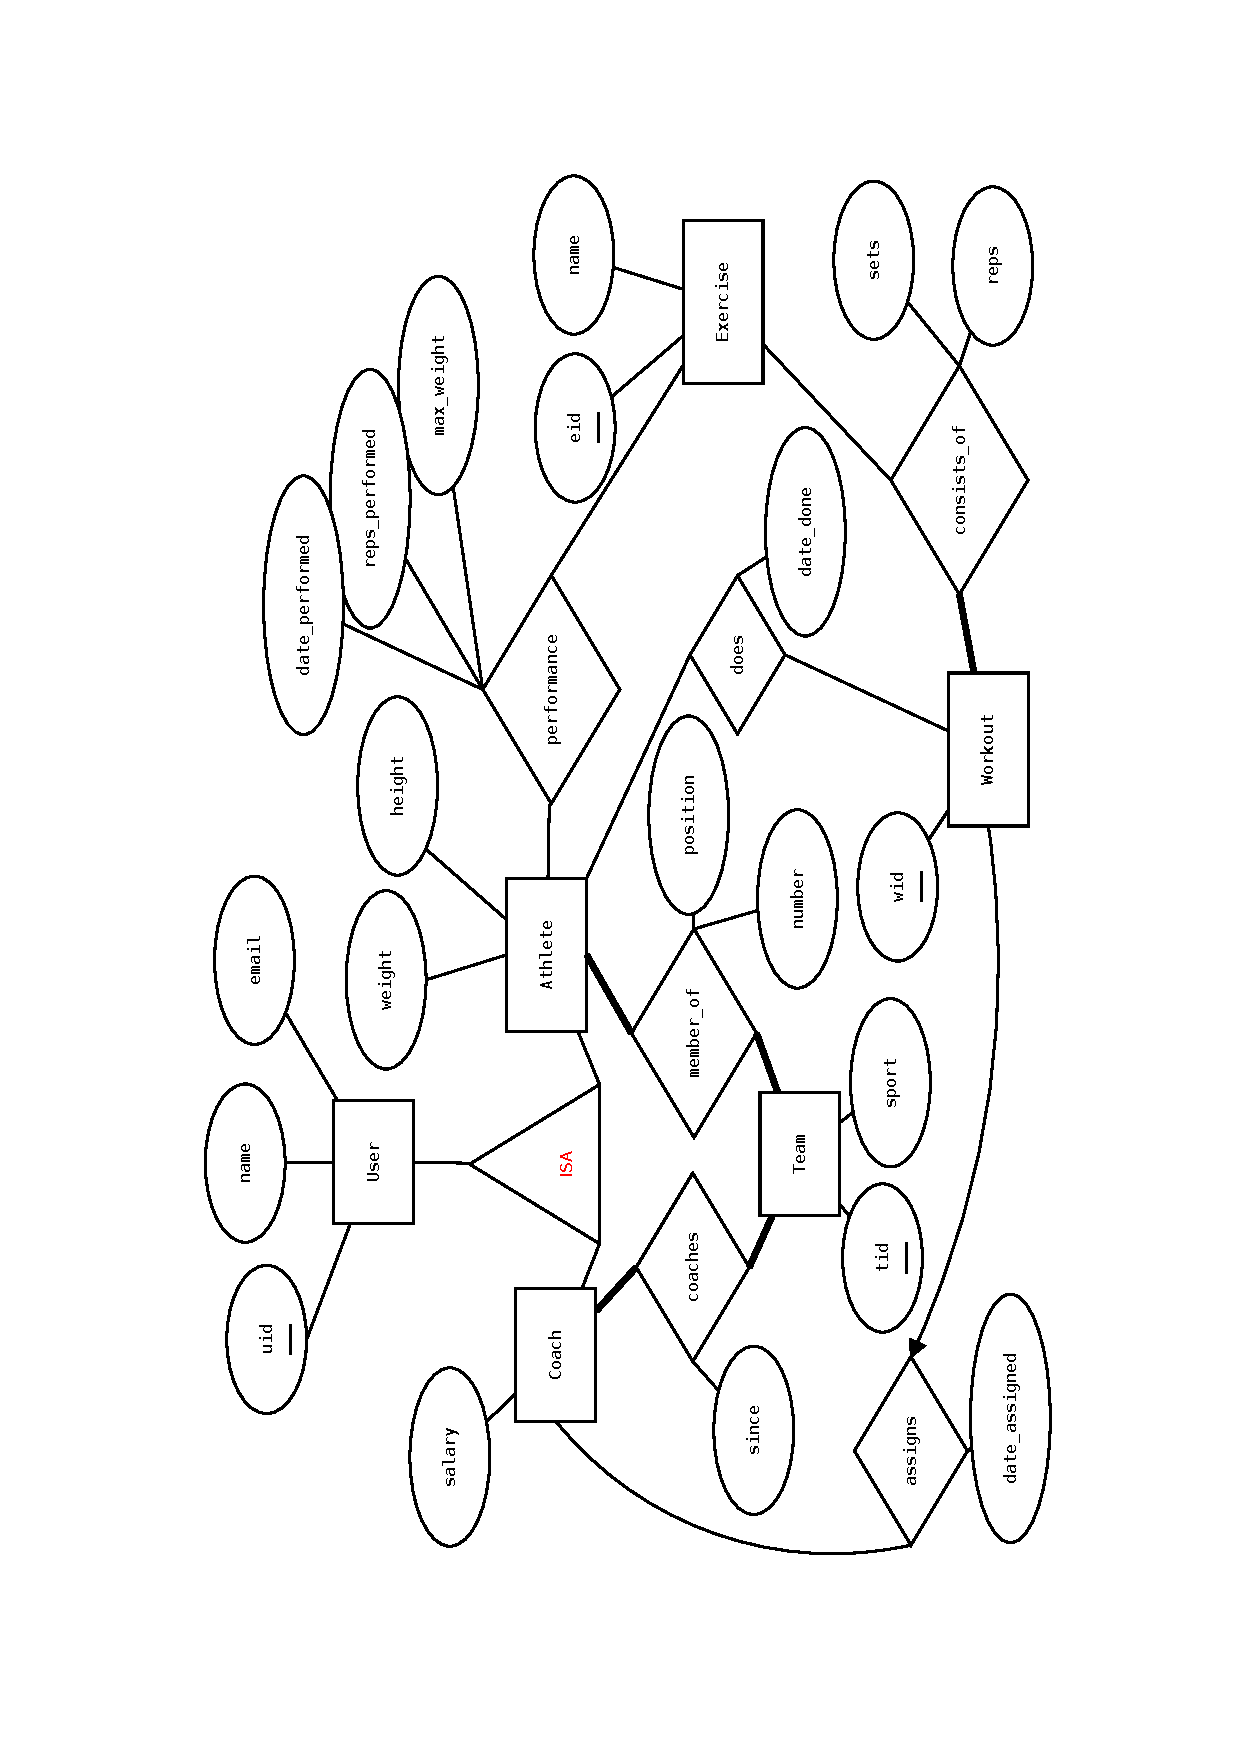
\includegraphics{erdiagram.pdf}

\end{document}
